\chapter{相关理论与技术}
本章介绍在基于海量数据挖掘的出租车移动模型的研究和实现中所涉及的相关理论与技术,这些理论和技术为本文后续模型设计、算法设计和原型系统构建提供参考依据。首先介绍车联网以及其中通信机制的实现原理;其次海量交通数据挖掘技术,明确数据挖掘的研究内容;最后介绍机会网络仿真技术,为协议的仿真验证提供有力支持。


\section{车联网概述}
车联网(Internet of Vehicles)是以车辆作为节点,利用传感器,车辆位置,车载wifi等构成的动态网络。

在车联网的研究当中,有一类我们称之为移动容断网络(DTMN,Delay Tolerant Mobile Network),这种网络主要指车载网络、战术网络等移动节点组成的网络,其较普通的DTN具有节点移动性更强的特点,也更加符合以上所述的应用场景。由于节点的移动性导致网络频繁割裂,连接频繁中断,消息传输的源节点到消息传输的目的节点之间没有端到端的连接。目前的研究者在解决上述问题时,通常使用“存储-携带-转发”(Store-Carry-Forward)[42]机制代替传统的“存储-转发”(Store-Forward)机制来完成消息的传递。

\begin{figure}
\centering
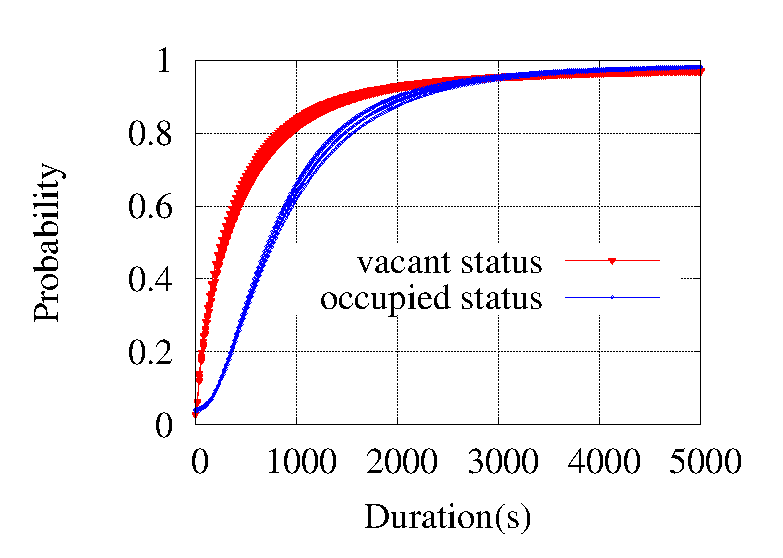
\includegraphics[width=0.5\textwidth]{figures/assumption/durationdis.eps}\\
\caption{状态持续时长分布}\label{figure_vehicles_network}
\end{figure}

如图 3所示,在移动容迟网络中,节点S期望将消息传递到节点D,但是网络中并不存在从S到D的链路,消息只能靠节点间的移动而相互传播,最终投递到D,而担任消息携带及转播角色的节点为全网内所有节点F。

\section{海量交通数据挖掘技术}
\section{ONE仿真技术}
芬兰赫尔辛基工业大学开发了一款专门用于仿真间断连通的机会网络的软件,叫做 机会网络仿真平台[59](Opportunistic Networking Environment,ONE)。该平台可以用来对DTN网络路由进行全面的仿真,因为它提供了一整套网络模拟的框架。在底层提供了各式节点移动的模型,可以模拟节点的移动。在网络层提供了各式路由的模型,可以模型报文的产生与交换。此外还有较为完整且可以自定义的报告模块,可以有针对性地扩展自己需要的路由性能指标的统计和计算。ONE还支持可视化的运行界面和命令行的运行界面,方便用户操作、配置和分析。图 6为ONE的结构图。
仿真平台ONE的主要组成和运行机制如下:

\subsection{移动模型}
ONE中主要包括三种基本的节点移动模型:随机的移动,受限于地图的移动,以及依据外部数据的移动。其中,随机的移动主要包括随机游走、随机路点等模型。受限于地图的移动包括规定路线,或受限于路网结构的随机移动等。而基于外部数据的移动将利用到ONE加载外部数据的接口。仿真引擎在仿真时,调用移动模型确定下一时刻的节点位置、方向、速度等属性,而移动模型就根据自身的特性多态地返回这些数据给仿真引擎,从而达到了节点移动与其他特性的解耦。同时,这也为移动模型和移动方式的扩展带来了极大的方便。图 7给出了ONE移动模型模块的组成。

\subsection{路由模型}
与节点移动模块的设计思路相同,消息路由模块的设计思路也是利用多态的方法。仿真引擎在仿真时,调用路由模块基类的抽象方法,而实际选择的路由策略将会根据自身的特点返回给仿真引擎相应的路由策略的选择情况。在路由策略中,主要分为主动路由和被动路由两大类,而现有的常用的路由策略均继承自主动路由。ONE自带了一些常用的路由策略,如直接交付路由Direct Delivery、喷射等待路由Spray-and-Wait、传染病路由Epidemic、等。在同一次仿真中,同时,ONE支持新的路由协议的开发,本文即根据其仿真引擎的规范,扩展了一套全新的路由协议,并在仿真引擎的帮助下完成了协议的仿真验证工作。图 8给出了ONE路由模块的组成。

\subsection{统计报告}
ONE提供了报告模块,利用侦听记录并统计所有事件,在仿真结束后将各项数值的统计结果按照既定的算法进行计算,得到需要的指标。ONE提供报告模板的自定义功能,可以根据需要制定各项指标的计算方法,这样在仿真结束后就能统计并输出需要的性能指标。在路由协议的仿真中,常用的统计指标有报文传输延迟、传输成功率、节点联系次数、节点间连接时间等。图~`9给出了ONE统计报告模块的组成。

\subsection{仿真引擎}
ONE的仿真引擎主要有两种运行方式,分别是命令行形式的批处理运行和GUI形式的单个配置运行。利用GUI形式运行可以清楚地看到节点的移动,消息的路由以及事件、报告的产生,方便调试和配置参数。利用批处理形式运行可以一次性得到大量的仿真结果,方便后期对报告的处理,进一步得到性能指标。图 10为ONE以GUI形式运行的截图,而图 11是ONE以批处理形式运行的截图。

本文将选用ONE作为仿真验证平台,因为ONE是专门为DTN路由协议的仿真设计实现的仿真平台,有丰富的系统接口和完善的功能。本文在仿真验证上需要对该平台进行二次开发,因为该平台目前尚不支持多播协议,需要对底层数据结构进行调整,配置相应的消息事件生成模块、报表统计模块,同时扩展路由协议模块,实现本文提出的协议与若干待比较的协议,最后利用ONE的仿真引擎完成仿真模拟,对统计结果进行分析对比,获得性能评估结果。

\section{本章小结}

本章给出了与本论文相关的理论和技术,包括移动容迟网络技术以及多播路由技术,它们是本文第三章和第四章中算法的核心理论基础,前者为第三章中模型的设计与第四章中缓存管理算法提供理论基础,后者为第三章的运动趋势辅助的多播路由概念模型提供理论基础;仿真平台ONE是本课题采用的仿真验证工具,用来对原型系统进行仿真验证。

